We will now proceed to describe our tool in more detail. The core part of the Python library is a function that generically searches for secure parameters for both LWE and SIS instances, as well as for ring and module variants. Moreover, some schemes depend on the statistical security of either LWE or SIS. We hence include classes to find parameters satisfying this criteria as well as basic variants of LWE and SIS. % TODO: maybe not here just in the section. 
Furthermore, we provide a set of utility classes and methods for the most used distributions and norms.
A configuration class allows for a substantial customization of the estimation process.
The tool can either estimate the bit security level of fixed parameter sets or generically search for parameter sets that satisfy a certain bit security level.

% class for distributions... from section this modelling, problems, generic search... Überblick, wie verwendbar,
% automatische norm umwandlung,
% sonstige features
\section{Supported Distributions} \label{sec:supported-distributions}% TODO
The secret distribution used in encryption schemes based on LWE or SIS can be either distributed according to a Gaussian or a uniform distribution. The error distribution in LWE must be a Gaussian distribution with parameter $\alpha$. In general, if both error and secret in LWE are sampled according to Gaussian distributions, their parameters may differ. Currently, however, the \textit{estimator} only supports secrets that follow a uniform distribution or a Gaussian distribution with the same parameter as the error distribution.

\subsection{Gaussian Distribution}\label{sec:gaussian-bounds}
In some applications, we receive a Gaussian distribution as input but require a bound in some norm to estimate the hardness of an SIS instance. Hence, we need to transform a Gaussian with parameter $s  = \sqrt{2 \pi} \sigma$ into a bound $\beta$ given some security parameter $\texttt{sec}$. Note that a $n$-dimensional Gaussian $D_{\mathbb{Z}^n, s}$ can be sampled by combining samples from $n$ independent one-dimensional Gaussians $D_{\mathbb{Z}, s}$ \cite{GJS15}. %TODO check

For a Gaussian distribution and a random variable $X$ with $X \sim D_{\mathbb{Z}, s}$, the following inequality holds for any $k>0$ with $\beta = k\sigma$ \cite[Lemma~4.4]{Lyu12}: % put as theorem, also for norm inequalities

\begin{align}
    \text{Pr}\left[ |X| > k\sigma \right] \leq 2 e^{\frac{-k^2}{2}} & \iff \text{Pr}\left[ |X| > \beta \right] \leq 2 e^{\frac{-\beta^2}{2\sigma^2}} \\
                                                                    & \iff \text{Pr}\left[ |X| > \beta \right] \leq 2 e^{\frac{-\pi \beta^2}{s^2}}   \\
\end{align}

We demand $2 e^{-\pi \beta^2/s^2} \leq 2^{-\texttt{sec}}$  and obtain

\begin{align*}
    2 e^{-\pi \beta^2/s^2}   \leq 2^{-\texttt{sec}} & \iff       -\pi \frac{\beta^2}{s^2} \leq (-\texttt{sec} - 1)\ln (2)                \\
                                                    & \iff \beta                    \geq s \sqrt{\frac{(\texttt{sec} + 1) \ln(2)}{\pi}}.
\end{align*}

\begin{theorem}[Gaussian to Bound]\label{th:gaussian-bound}
    Given a Gaussian distribution $D_{\mathbb{Z}^n, s}$ with width parameter $s  = \sqrt{2 \pi} \sigma$ and a security parameter $\texttt{sec}$, we can compute a bound $\beta$ such that a sample $\mathbf{v}$ drawn from $D_{\mathbb{Z}^n, s}$ satisfies $\text{Pr}\left[ \|\mathbf{v}\|_\infty \geq \beta \right] \leq 2^{-\texttt{sec}}$ as follows:
    \begin{equation}
        \beta  = s \sqrt{\frac{(\texttt{sec} + 1) \ln(2)}{\pi}}.
    \end{equation}
\end{theorem}

Analogously, if we require a bound in the $\ell_2$-norm, we have that $\text{Pr}\left[ \|X\|_2 > k\sigma \sqrt{n} \right] \leq k^n e^{\frac{n}{2}(1-k^2)}$, for an $n$-dimensional Gaussian $D_{\mathbb{Z}^n, s}$ and a random variable $X$ with $X \sim D_{\mathbb{Z}^n, s}$, for any $k>1$ \cite[Lemma~4.4]{Lyu12}. We set $k=\sqrt{2}$ and obtain

\begin{align*}
    \text{Pr}\left[ \|X\|_2 > \sigma \sqrt{2n} \right] \leq 2^{\frac{n}{2}} e^{\frac{n}{2}(1-2)} & = 2^{\frac{n}{2}} 2^{-\log e \frac{n}{2}} \\
                                                                                                 & = 2^{\frac{n}{2}(1 -\log e)}
\end{align*}
If $2^{\frac{n}{2}(1 -\log e)} \leq 2^{-\texttt{sec}}$, we take $\sigma \sqrt{2n}$ as our bound $\beta$. Otherwise, we bound the $\ell_2$-norm of $\beta$ by the $\ell_\infty$-norm bound from \cref{th:gaussian-bound} as described in \cref{sec:norm-bounds}.

We provide the classes $\texttt{GaussianAlpha}$, $\texttt{GaussianSigma}$ and $\texttt{GaussianS}$ to allow for the most flexibility in specifying a Gaussian distribution.

\subsection{Uniform Distribution}
For uniform distributions, we support all distributions that are supported by the \textit{estimator}, namely, uniform modulo $q$, uniform in the interval $[a,\dots,b]$ and a sparse uniform distribution with parameters $((a,b), h)$, where exactly $h$ components are in the interval $[a,\dots,b] \setminus \{0\}$ and all other components are zero. Note that we only consider discrete distributions are over $\mathbb{Z}$.

We can estimate the corresponding standard deviation for a Gaussian distribution by computing the variance of the uniform distribution. Given a lower and upper bound $(a, b)$, the variance for a discrete uniform distribution is defined as $\sigma^2 = \frac{(b - a + 1)^2 - 1}{12}$. For a uniform distribution modulo $q$ we set $a = -\left\lfloor \frac{q}{2} \right\rfloor, b = \left\lfloor \frac{q}{2} \right\rfloor$.

For a sparse discrete $n$-dimensional uniform distribution $\mathcal{U}_h$ with an additional sparseness parameter $h$ and a random variabel $X \sim \mathcal{U}_h$, we can compute the expected values $\mathbb{E}(X^2)$ and $\mathbb{E}(X)^2$ as follows \cite{APS15}:
% TODO maybe figure out why that is so

\begin{align}
    \mathbb{E}(X^2) & = \frac{h}{n} \cdot \frac{2b^3 + 3b^2 + b - 2a^3 + 3a^2 - a}{6(b - a)} \\
    \mathbb{E}(X)^2 & = \frac{h}{n} \cdot \frac{b (b + 1) - a(a - 1)}{2(b - a)}
\end{align}

and obtain the variance $\text{Var}(X) = \mathbb{E}(X^2) - \mathbb{E}(X)^2$.



\section{Norm Bound Inequalities} \label{sec:norm-bounds}% TODO: check
%TODO: write some prose about why we need that
% TODO: make sure that it is clear that these are bounds!!!
In practical scenarios, oftentimes we require that the bound of a result does not exceed a certain value to guarantee correctness. In addition, we have seen that estimation algorithms rely on bounds in different $\ell_p$-norms. For example, the combinatorial attack in \cref{sec:combinatorial} needs a bound in $\ell_\infty$ norm, whereas the dual attack in \cref{sec:dual-attack} uses bounds in the Euclidean norm. We thus need a way to bound a value of a bound in one norm by a value in a different norm. In our tool, we define a norm class with parameter $p$ and provide a  method $\texttt{to\_Lp()}$ for conversions into all other norms mentioned here. We begin by the following Theorem.
\begin{theorem}\label{th:norm-rel1}
    Let $f \in \mathcal{R}_q$ with $f = \sum_i f_i X^i$ as in in \cite{BDLOP18} and $p, q \in \mathbb{N}$ with $\infty \geq p \geq q \geq 1$. Then the following inequation holds:
    \begin{align}
        \| f \|_p & \leq \| f \|_q \label{eq:norm-inf-leq-1}.
    \end{align}
    Let $p, q \in \mathbb{N}$ with $1 \leq p \leq q \leq \infty$. Then the following inequation holds:
    \begin{align}
        \lim_{q' \rightarrow q}\| f \|_p & \leq \lim_{q' \rightarrow q} n^{\frac{1}{p} - \frac{1}{q'}}\| f \|_{q'} \label{eq:norm-1-leq-inf}.
    \end{align}
\end{theorem}
It is easy to see from the definition of the norms in \cref{sec:norms} that \cref{eq:norm-inf-leq-1} is true. \cref{eq:norm-1-leq-inf} follows from Hölder's inequality. We proof the statement in \cref{sec:proof-norm}.

In addition, oftentimes we consider norms in the canonical embedding. Let $\mathcal{O}_K$ be the ring of integers of a number field $K=\mathbb{Q}(\theta)$, where $\theta$ is an algebraic number and $\sigma$ denote the canonical embedding as defined in \cite{DPSZ12}. Then, according to \cite[Theorem~7]{DPSZ12} for $f \in \mathcal{O}_K$  the following inequations hold: % TODO: why?
\begin{align}
    \| f \|_\infty         & \leq \| \sigma(f) \|_\infty \label{norm5}, \\
    \| \sigma(f) \|_\infty & \leq \| f \|_1 \label{norm6}.
\end{align}
(We assume that the constant $C_m$ used in the original Theorem is $1$ for $m$ a power of $2$ \cite[Lemma~3]{DPSZ12}.) If we combine \cref{norm5,norm6} respectively with \cref{eq:norm-1-leq-inf} we obtain the following theorem.
\begin{theorem}\label{th:norm-rel2}
    Let $f \in \mathcal{O}_K$ as in in \cite{DPSZ12}. Then, the following two inequations hold:
    \begin{align}
        \| \sigma(f) \|_\infty & \leq \| f \|_1 \leq n^{1 - \frac{1}{p}} \| f \|_p \text{ for } p \geq 1, \text{ and } \label{eq:Coo-norm}                  \\
        \| f \|_p              & \leq  n^{\frac{1}{p}} \| f \|_\infty \leq n^{\frac{1}{p}} \| \sigma(f) \|_\infty \text{ for } p \leq \infty  \label{norm7}
    \end{align}
\end{theorem}
We can thus bound a given bound in the norm $\ell_q$ for some $q$ by a bound in some $\ell_p$ norm using the above inequalities and analogously in the embedding norm, which we call $\mathcal{C}_p$. We combine both results in the method $\texttt{to\_Lp()}$ and $\texttt{to\_Cp()}$ in the norm classes $\texttt{Lp}$ and $\texttt{Cp}$ respectively. Note that the embedding norm $\mathcal{C}_p$ works internally like the $\ell_p$ norm, as we define both for vector spaces of dimension $n$. We merely need the results in \cref{th:norm-rel2} for the conversion between both norms.

We also want to be able to estimate bounds on the result of addition and multiplication of vectors of a bounded length in different norms. Note that the degree of the polynomial of the underlying ring to which we apply the norms must match. For addition, we simply bound the second addend by the used norm of the first as described in \cref{th:norm-rel1,th:norm-rel2} and add both bounds to obtain a bound on the result in the norm of the first addend. It is slightly more complicated for multiplication, and we state the results in the next theorem.

\begin{theorem}[Multiplication of Norm Bounds \cite{BDLOP18, DPSZ12}]\label{th:mult}
    Let $f$ be defined as above and let $g \in \mathcal{R}_q$ where $g = \sum_i \overline{g}_i X^i$ where $g_i \in \left[-(q-1)/2, (q-1)/2\right]$ and $\overline{g}_i = g_i \mod q$ as in \cite{BDLOP18}. We then can define the following inequations for multiplication according to \cite{BDLOP18}:

    \begin{equation}\label{eq:mult1}
        \begin{aligned}
            \|f \cdot g\|_\infty & \leq \|f\|_\infty \cdot \|g\|_1, \\
            \|f \cdot g\|_\infty & \leq \|f\|_2 \cdot \|g\|_2.
        \end{aligned}
    \end{equation}

    Let $x, y \in \mathcal{O}_K$. Then, the following inequation holds according to \cite{DPSZ12}:
    \begin{align}
        \| \sigma(x \cdot y) \|_p & \leq  \| \sigma(x) \|_\infty \cdot \| \sigma(y) \|_p. \label{eq:mult4}
    \end{align}
    (Again, we assume that $C_m = 1$ in the original statement.)
\end{theorem}

If \cref{eq:mult1} does not apply and the bounds for both vectors that we want to multiply is given in some $\ell_p$-norm, we simply convert both bounds to the $\mathcal{C}_\infty$-norm as described in \cref{eq:Coo-norm} and apply \cref{eq:mult4} with $p=\infty$. In the case that we have an $\ell_p$-norm and a $\mathcal{C}_q$-norm for some $p,q$, we similarly convert the $\ell_p$-norm to the $\mathcal{C}_\infty$-norm and apply \cref{eq:mult4}. If both bounds are $\mathcal{C}_p$-norm bounds with $p < \infty$, we apply \cref{eq:mult4} twice, once with the first bound converted to the $\mathcal{C}_\infty$-norm and once with the second norm converted to the $\mathcal{C}_\infty$-norm, and take the best value as our result bound.


\section{Problem Classes}\label{sec:problem-classes}
We now present the problem classes in $\texttt{lattice\_parameter\_estimation/problem}$ (see \cref{fig:problem-classes}).
\begin{figure}[h]
    \centering
    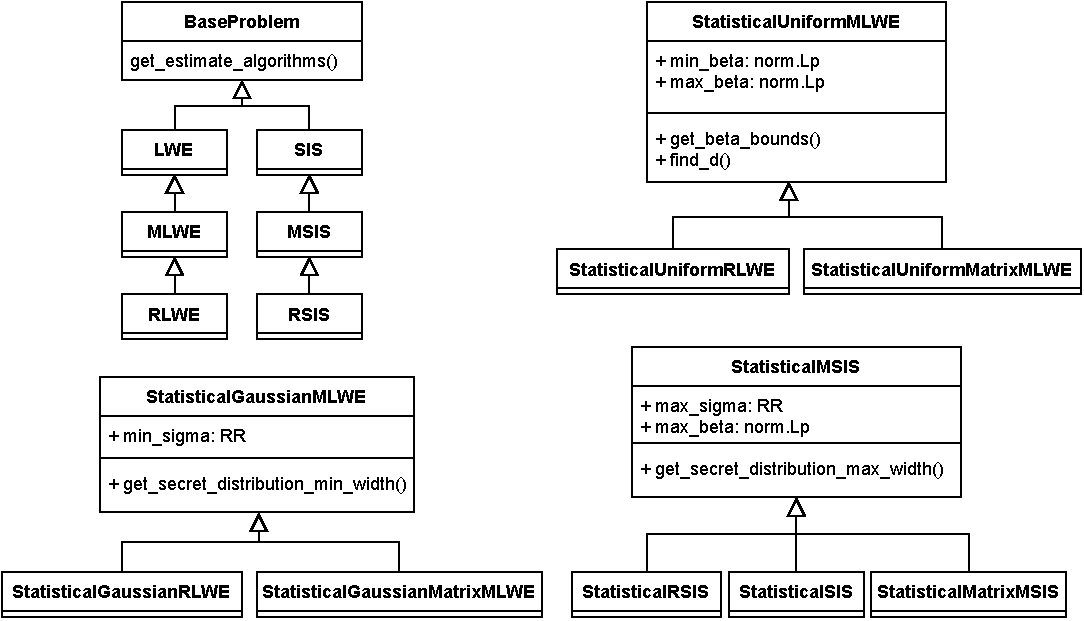
\includegraphics[width=1\textwidth]{graphics/problem_classes.pdf}
    \caption{Problem classes}\label{fig:problem-classes}
\end{figure}
$\texttt{LWE}$ and $\texttt{SIS}$ inherit from the base class $\texttt{BaseProblem}$. All instances provide a method $\texttt{get\_estimate\_algorithms()}$ that returns a list of algorithm instances that can be executed by the function $\texttt{estimate()}$. Furthermore, any instance of $\texttt{BaseProblem}$ can be compared to a bit security level (for more details, we refer the reader to the documentation). The $\texttt{LWE}$ class is initialized by the secret dimension $n$, a modulus $q$, the number of samples $m$, a $\texttt{secret\_distribution}$ and a $\texttt{error\_distribution}$. Both $\texttt{secret\_distribution}$ and $\texttt{error\_distribution}$ must be instances of the class $\texttt{distributions.Distribution}$. Instead of $\texttt{secret\_distribution}$ and $\texttt{error\_distribution}$, a bound of type $\texttt{norm.BaseNorm}$ must be set for $\texttt{SIS}$. Note that both $\texttt{distributions.Uniform}$ and $\texttt{distributions.Gaussian}$ are instances of $\texttt{norm.BaseNorm}$ and can thus be used as a bound. We compute the bound for a given distribution instance as described in \cref{sec:supported-distributions}.

For ring and module variants $\texttt{RLWE}$, $\texttt{RSIS}$ and $\texttt{MLWE}$, $\texttt{MSIS}$ respectively, $n$ denotes the degree of the polynomial of the underlying ring $\mathcal{R}_q$. The module variants $\texttt{MLWE}$ and $\texttt{MSIS}$ take an addition parameter $d$ for the rank of the module.

While there exist special cases where the ring structure of problem instances can be exploited in an attack on LWE or SIS, % TODO: find examples
in general, the hardness of ring and Module variants is estimated by interpreting the coefficients of elements of $\mathcal{R}_q$ as vectors in $\mathbb{Z}_q^n$ \cite{ACDDPPVW18}. If we take into account the considerations we presented in \cref{sec:ring-module}, we can thus reduce ring and Module instances, when calling $\texttt{get\_estimate\_algorithms()}$ on the ring and module variant of $\texttt{LWE}$ and $\texttt{SIS}$, as follows:
\begin{itemize}
    \item RLWE$_{n, q, m, \chi} \longrightarrow$ LWE$_{n, q, m \cdot n, \chi}$
    \item MLWE$_{n, d, q, m, \chi} \longrightarrow$ LWE$_{n \cdot d, q, m \cdot n, \chi}$
    \item RSIS$_{n, q, m, \beta} \longrightarrow$ SIS$_{n, q, m \cdot n, \beta}$
    \item MSIS$_{n, d, q, m, \beta} \longrightarrow$ SIS$_{n \cdot d, q, m \cdot n, \beta}$
\end{itemize}


In addition to the base problem variants, we define some statistically secure variants for both LWE and SIS, since some schemes depend on the unconditional hardness of either LWE or SIS. More precisely, we ask for parameters such that an arbitrary powerful attacker can only break the scheme with probability less than $2^{-\texttt{sec}}$.

\paragraph{$\texttt{StatisticalGaussianMLWE}$.} For LWE, we define a statistically secure variant over a Gaussian distribution and over a uniform distribution. $\texttt{StatisticalGaussianMLWE}$ follows Corollary 7.5 and Theorem 7.4 in \cite{LPR13}. The mapping of the parameters in \cite{LPR13} to the usage in this work can be found in \cref{tab:mapping-LPR13}. We obtain the following theorem:

\begin{theorem}[Statistically Secure MLWE Over a Gaussian Distribution {\cite[Corollary~7.5]{LPR13}}]
    Let $\mathcal{R}$ be the ring of integers in the $m'$th cyclotomic number field $K$ of degree $n$, and $q \geq 2$ an integer.
    For positive integers $m \leq m + d \leq \text{poly}(n)$, let $\mathbf{A} = [ \mathbf{I}_{[m]} \mid \bar{\mathbf{A}}] \in (\mathcal{R}_q)^{[m] \times [m+d]}$, where $\mathbf{I}_{[m]} \in (\mathcal{R}_q)^{[m] \times [m]}$ is the identity matrix and $\bar{\mathbf{A}} \in (\mathcal{R}_q)^{[m] \times [d]}$ is uniformly random.
    Then with probability $1 - 2^{-\Omega(n)}$ over the choice of $\bar{\mathbf{A}}$, the distribution of $\mathbf{A}\mathbf{x} \in (\mathcal{R}_q)^{[m]}$, where each coordinate of $\mathbf{x} \in (\mathcal{R}_q)^{[m+d]}$ is chosen from a discrete Gaussian distribution of parameter $s > 2n \cdot q^{m / (m+d) + 2/(n (m+d))}$ over $\mathcal{R}$, satisfies that the probability of each of the $q^{n m}$ possible outcomes is in the interval $(1 \pm 2^{-\Omega(n)}) q^{-n }$ (and, in particular, is within statistical distance $2^{-\Omega(n)}$ of the uniform distribution over $(\mathcal{R}_q)^{[m]}$). % TODO change [x]times[y] notation???
\end{theorem}
% TODO: anything more? can you provide an intuition?

If a security parameter is passed and $\texttt{sec} > n$, we raise an exception.
The resulting minimal standard deviation is stored in the instance variable $\texttt{min\_sigma}$ and the corresponding distribution can be obtained by calling $\texttt{get\_secret\_distribution\_min\_width()}$ on the class instance.



\paragraph{$\texttt{StatisticalUniformMLWE}$.} The authors of \cite{BDLOP18} describe statistically secure MLWE instances over a Uniform distribution with invertible elements. The samples $(\mathbf{A}', h_{\mathbf{A}'}(y))$ of the resulting MLWE instance are within statistical distance $2^{-\texttt{sec}}$ of $(\mathbf{A}', \mathbf{u})$ for uniformly distributed $\mathbf{u}$. % TODO: check formulation

We obtain the following theorem (for a mapping of the parameters, see \cref{tab:mapping-BDLOP18}): %TODO 

\begin{theorem}[Statistically Secure MLWE Over a Uniform Distribution {\cite[Lemma~4]{BDLOP18}}]
    Let $1 < d_2 < n$ be a power of 2. If $q$ is a prime congruent to $2d_2 + 1 \;(\text{mod } 4d_2)$ and
    \begin{equation}
        q^{m/(m+d)} \cdot 2^{2 \texttt{sec}/((m+d)\cdot n)} \leq 2 \beta < \frac{1}{\sqrt{d_2}} \cdot q^{1/d_2}
    \end{equation}
    then any (all-powerful) algorithm $\mathcal{A}$ has advantage at most $2^{-\texttt{sec}}$ in solving $\text{DKS}_{m,m+d,\beta}^\infty$, where $\text{DKS}^\infty$ is the decisional knapsack problem in $\ell_\infty$-norm.
\end{theorem}
Note that we replaced the fixed value of $128$ in the original Lemma with $\texttt{sec}$. The proof is essentially the same as in \cite{BDLOP18} and we will therefore refrain from stating it again here.


Hence, we have:
\begin{align}
    \beta_{min} & = \frac{q^{m/(m+d)} \cdot 2^{2 \texttt{sec}/((m+d)\cdot n)}}{2} \\
    \beta_{max} & = \frac{1}{2\sqrt{d_2}} \cdot q^{1/d_2} - 1
\end{align}
% TODO: explain how to arrive at 2*\texttt{sec} instead of 256, für generellen \texttt{sec} parameter ...
% proof zum Beispiel im Anhang ...

The variable $d_2$ can be passed as an argument. If it is not passed, we try to find $d_2$ by iterating over all powers of $2$ that are smaller than $n$.
The resulting bounds are converted to $\ell_\infty$ and stored in the instance variables $\texttt{min\_beta}$ and $\texttt{max\_beta}$. We also provide an instance method $\texttt{get\_beta\_bounds()}$ to obtain a tuple of both.

For both statistically secure MLWE variants, we include the corresponding ring versions $\texttt{StatisticalGaussianRLWE}$ and $\texttt{StatisticalUniformRLWE}$ for $d=1$ and matrix versions $\texttt{StatisticalGaussianMatrixMLWE}$ and $\texttt{StatisticalUniformMatrixMLWE}$ for which the width and height of the matrix $\mathbf{A}$ in \cite{LPR13} can be passed instead of $m$ and $d$. % TODO: include instead of included?
% TODO: explain why this doesn't work for LWE


\paragraph{$\texttt{StatisticalMSIS}$.} We can find parameters for a statistically secure MSIS instance by following Section 4.1 of \cite{DOTT21}. The mapping of the parameters in \cite{DOTT21} is shown in \cref{tab:mapping-DOTT21}. More specifically, we ask to find a MSIS instance where the probability that non zero elements $\mathbf{r}$ in the Euclidean ball $B_{m}(0, 2B)$ satisfy $\hat{\mathbf{A}}_1 \cdot \mathbf{r} = \mathbf{0}$ is smaller than $2^{-\texttt{sec}}$. % TODO check that this is not a quote

The number of elements in $B_{m+d}(0, 2B)$ can be estimated from above as $|B_{m+d}(0, 2B)| \ll (2 \pi e /((m+d) n))^{(m+d) n/2} \cdot (2 B)^{(m+d) n}$. The scheme is statistically binding if the probability that non zero elements in $B_{m+d}(0, 2B)$ of radius $2B$ in $\mathcal{R}_q^{m+d}$ map to $\mathbf{0}$ in $\mathcal{R}_q^{m}$ is negligible. Hence, it must hold that $|B_{m+d}(0, 2B)|/q^{m n} \leq 2^{-\texttt{sec}}$ and we get:

% TODO: look for bound of ball without o(...) if change also change in docstring, check out wikipedia => heuristic. maybe find version not heuristic?
% add that this is approximation, see https://en.wikipedia.org/wiki/Volume_of_an_n-ball
% for small n?

\begin{align}
    \left(\sqrt{\frac{2 \pi e}{(m+d) \cdot n}} \cdot 2 B\right)^{(m+d) \cdot n} & \leq 2^{-\texttt{sec}} \cdot q^{m\cdot n}                                                                       \\
    B                                                                           & \leq 2^{\frac{-\texttt{sec}}{(m+d)\cdot n} - 1} \cdot q^\frac{m}{m+d} \cdot \sqrt{\frac{(m+d)\cdot n}{2 \pi e}}
\end{align}

We convert the bound $B$ to a Gaussian over $\ell_2$-norm by following the procedure described in \cref{sec:gaussian-bounds}: % TODO: add appropriate reference

\begin{equation}
    s  \approx B \sqrt{\frac{\pi}{(\texttt{sec} + 1) \ln(2)}}
\end{equation}

% TODO: rephrase to obtain a lemma?
The resulting parameters $B$ and $s$ can be accessed by the instance variables $\texttt{max\_sigma}$ and $\texttt{max\_beta}$ or by calling $\texttt{get\_secret\_distribution\_max\_width()}$ on the class instance.

As for statistically secure MLWE, we again include a matrix version $\texttt{StatisticalMatrixMSIS}$ and a ring $\texttt{StatisticalRSIS}$ by setting $d=1$. In addition, the proof also applies to the base SIS variant and hence we include $\texttt{StatisticalSIS}$. Here, the height of the matrix $n$ becomes the rank of the modulus in the MSIS instance, i.e., $d=n$, and the degree of the polynomial is $1$.

% TODO: include graphic for matrix version???


\section{Parameter Search}
The main functionality of our tool is to search for secure parameter sets given a set of problem instances and is encapsulated in the function $\texttt{param\_search.generic\_search()}$. It is also possible to directly estimate the cost of a list of parameter problems by calling the function $\texttt{problem.estimate()}$. For more details, we refer to the documentation.

The high-level idea of the search is presented in \cref{alg:generic-search}. We begin with an initial parameter set. We then create a list of problem instances generated by a $\texttt{parameter\_problem}$ function and estimate the cost of all instances in the list by calling $\texttt{problem.estimate()}$. If the list contains multiple SIS instances or multiple LWE instances, we first attempt to reduce the instances to the easiest problem instance respectively. The reduction is not exhaustive and is realized by a simple comparison of the parameters $n, q, m$ and $\alpha$ or bound $\beta$ according to the following intuitive hardness results. For LWE, we have that the larger $n$ and $\alpha$ are and the smaller $q$ and $m$ are, the harder the problem becomes. For SIS, the problem becomes harder for increasing $n$ and $q$ and decreasing $\beta$ and $m$. The function then generates a list of estimation algorithm instances for each remaining problem instance and the resulting list is executed by an algorithm executor. The list is ordered according to expected runtime and output quality of the specified algorithms (see \cref{sec:tool-algorithms}). If the estimation is configured to be parallel, the algorithms are split up into sublist and executed concurrently on multiple processors.
% TODO: include how, \cref{sec:problem-reduction} 
Once we find an insecure problem instance (i.e., the estimated attack cost in clock cycles is smaller than $2^{\texttt{sec}}$), we terminate the estimation procedure and $\texttt{estimate()}$ returns a result that is labeled insecure. We then use the $\texttt{next\_parameters}$ function to generate a list L of (multiple) new parameter sets from our current parameter set and sort each of the new parameter sets into an ordered list with duplicate detection. The order is defined by a $\texttt{parameter\_cost}$ function. In the next step, we retrieve the parameter set with the lowest cost from L and repeat the procedure until the cost estimation step returns a secure result. The result includes the estimates for all cost models and algorithms.

\begin{algorithm2e}
    \KwInput{sec, initial\_params, next\_parameters, parameter\_cost,  problem\_instance}

    L = OrderedList(initial\_params)\\
    \While{L $\neq \emptyset$}{
        current\_params = L.pop() \\
        instances = parameter\_problem(current\_params) \\
        result = estimate(instances, sec) \\
        \If{result is secure}{
            \Return{(result, current\_params)}\\
        }
        \Else{
            next\_param\_sets = next\_parameters(current\_params)\\
            \ForAll{param\_set in next\_param\_sets}{
                sort param\_set into L according to parameter\_cost function\\
            }
        }
    }
    \caption{Generic Search} \label{alg:generic-search}
\end{algorithm2e}


\section{Configuration Options}\label{sec:config-options}
The configuration of the estimation can be customized via the class $\texttt{algorithms.Configuration}$, which is passed as an optional argument of $\texttt{param\_search.generic\_search()}$.

We noted that the $\texttt{estimate()}$ function can be configured to run in parallel, which may speed up the search, in particular if many cost models need to be tested (e.g., with configuration setting $\texttt{conservative=False}$ and long running algorithms like $\texttt{ARORA\_GB}$, $\texttt{CODED\_BKW}$ and $\texttt{PRIMAL\_DECODE}$ are used (see \cref{sec:tool-algorithms}). The list of used algorithms can be changed in the configuration. We recommend to include at least $\texttt{PRIMAL\_USVP}$ for LWE instances and $\texttt{LATTICE\_REDUCTION}$ for SIS instances (as in the default configuration) to make full use of early termination, since the estimate algorithms for these attacks have a short runtime and yield relatively low cost estimates. A user can also specify a security strategy. We included three strategies, namely, $\texttt{ALL\_SECURE}$, $\texttt{SOME\_SECURE}$ and $\texttt{NOT\_INSECURE}$. For $\texttt{ALL\_SECURE}$, the search only terminates if all specified algorithms return a cost that satisfies the security level. Depending on the choice of algorithms, the search may not terminate since, for example, Arora-GB for larger $n$ takes too long and is therefore aborted once the timeout is reached and cannot return a cost estimate. $\texttt{SOME\_SECURE}$ demands that at least one algorithm returns a secure estimate for each problem instance for a given parameter set. $\texttt{NOT\_INSECURE}$ only demands that no algorithm returns an insecure cost. We recommend using $\texttt{SOME\_SECURE}$ (as in the default configuration).


\paragraph{Cost Models.} \label{sec:tool-costmodels} Attacks that use BKZ for lattice reduction require a cost model to estimate the number of CPU cycles in the SVP subroutine. Default cost models are shown in \cref{tab:costmodels}. We distinguish between estimates for classical, quantum, sieving and enumeration and each of these categories can be deselected by setting the respective parameter to $\texttt{False}$. At least one of classical and quantum and of sieving and enumeration respectively must be selected to make use of the default cost models.

Note that classical and quantum cost models cannot be directly compared with each other. The number of operations per second that can be executed by a quantum computer may be significantly smaller than for classical computers. % TODO add more?

If all are unselected, custom cost models must be specified and passed as an argument. We included an option of taking the most conservative estimate for each category combination for a more efficient parameter search or estimation. Furthermore, we assigned a priority value on an ordinal scale to each cost model, which enables us to first run cost models that yield a lower cost and thus terminate the estimation process earlier for an insecure parameter set. The priority values of the default cost models are derived from \cref{fig:costmodels}.
\begin{figure}[h!]
    \centering
    \begin{subfigure}{0.5\textwidth}
        \centering
        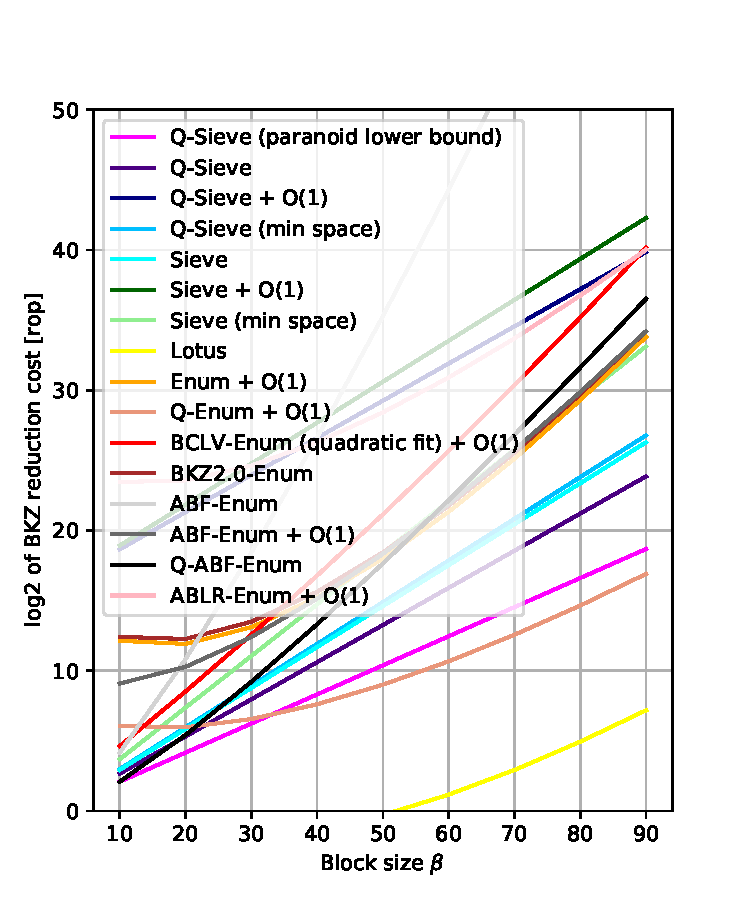
\includegraphics[width=1\textwidth]{graphics/cost_models.pdf}
        \caption{All}
    \end{subfigure}
    \begin{subfigure}{0.49\textwidth}
        \centering
        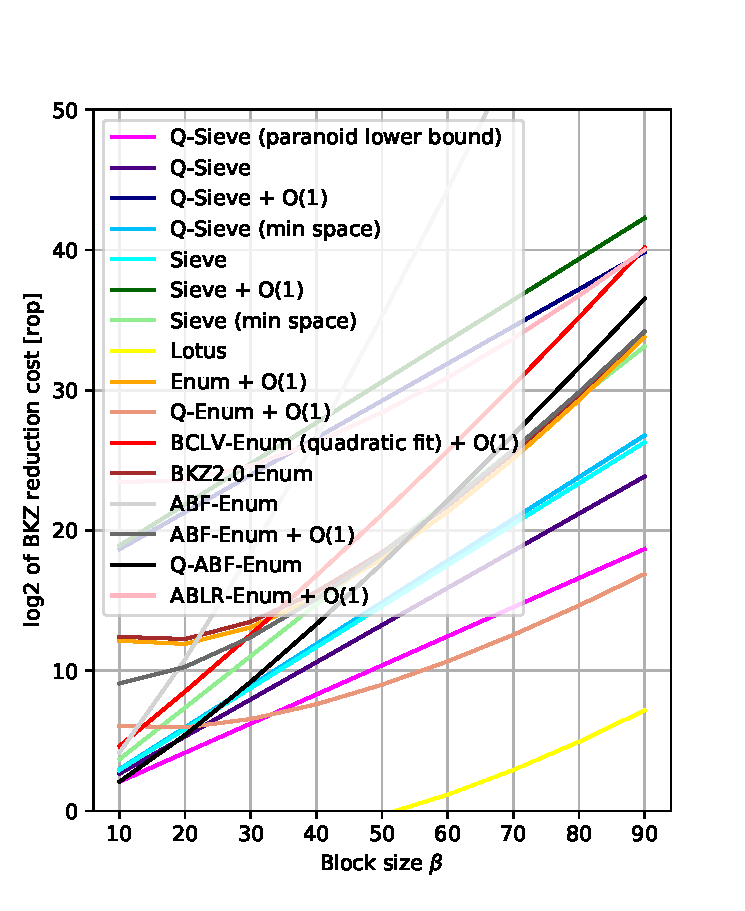
\includegraphics[width=1\textwidth]{graphics/cost_models_small_beta.pdf}
        \caption{Small block size $\beta$}\label{fig:costmodels-small-beta}
    \end{subfigure}
    \begin{subfigure}{0.5\textwidth}
        \centering
        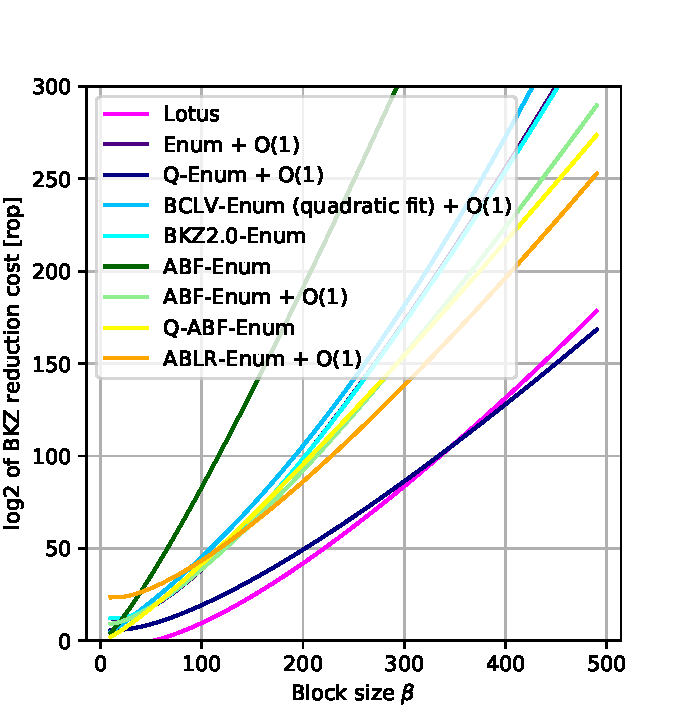
\includegraphics[width=1\textwidth]{graphics/cost_models_enum.pdf}
        \caption{Enumeration}\label{fig:costmodels-enum}
    \end{subfigure}
    \begin{subfigure}{0.49\textwidth}
        \centering
        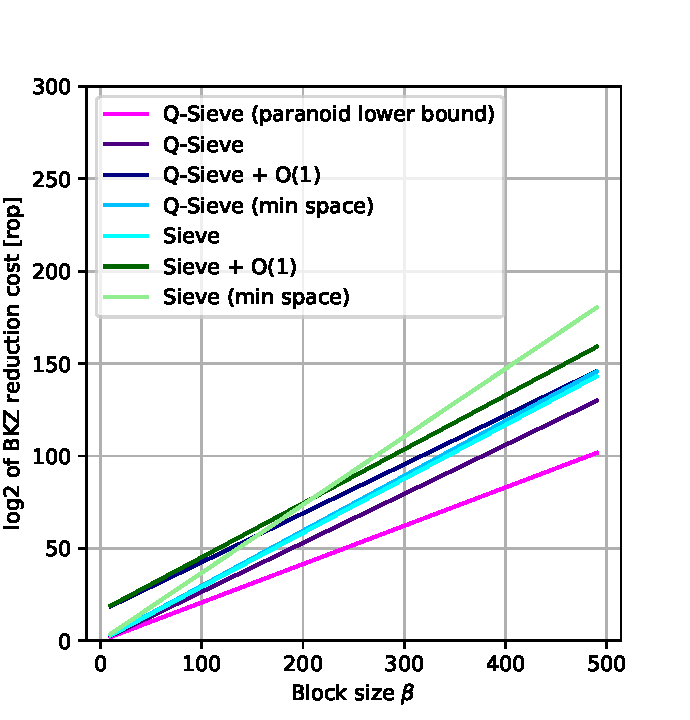
\includegraphics[width=1\textwidth]{graphics/cost_models_sieving.pdf}
        \caption{Sieving}\label{fig:costmodels-sieving}
    \end{subfigure}
    \caption{Cost models}\label{fig:costmodels}
\end{figure}
The number of BKZ rounds can be configured according to the more conservative Core-SVP model $\texttt{algorithms.BKZ\_SVP\_repeat\_core}$ \cite{ADPS16} in which the polynomial factor of the runtime complexity of BKZ is completely ignored. In addition, we provide a more realistic model $\texttt{algorithms.BKZ\_SVP\_repeat\_8d}$ for a BKZ cost of $8 \cdot d \cdot t_k$ BKZ rounds, where $d$ again referes to the lattice dimension and $t_k$ is the number of clock cycles required for the SVP subroutine (see \cref{sec:bkz-8d}). % TODO maybe add a little more of evaluation here


\paragraph{Algorithms.} \label{sec:tool-algorithms} \cref{fig:SIS-algs,fig:LWE-other-sigma,fig:LWE-Regev} show the plots of runtime and performance tests for the various algorithms that can be used in our tool. The parameters of SIS in \cref{fig:SIS-algs} are derived from \cite{MP12}, the parameters of LWE in \cref{fig:LWE-Regev} are based on \cite{Reg05}. We chose the parameters of \cref{fig:LWE-other-sigma}, such that most algorithms yield a result. Note that Arora-GB in \cref{fig:LWE-other-sigma} and Meet-in-the-Middle and Coded-BKW for higher dimensions in \cref{fig:LWE-Regev} return a cost of $\infty$ and therefore do not appear in the bit security plot. In \cref{fig:LWE-Regev}, computing the cost for Arora-GB for $n>512$ takes longer than the configured timeout of $200$s and does therefore also not show up in the plot. In accordance with the results, we assigned priority values on an ordinal scale to the estimation algorithms. In \cref{tab:lwe-alg-prio,tab:sis-alg-prio}, we present the list of algorithms and their corresponding priority values and justify our choice. Algorithms with a smaller priority value are expected to yield relatively good results quickly and can therefore be executed first. If the estimate result does not satisfy the specified security requirement, we can terminate the estimation process early in order to maximize the efficiency of our search. Note that, while convenient, directly comparing the results for different algorithms is not always admissible, as the compared algorithms may rely on different assumptions. Some algorithms may compute a more realistic cost, while others may return a more conservative or even paranoid cost estimate (e.g., BKZ is used with the Core-SVP paranoid lower bound). The results must be weighed carefully in order to guarantee the security of a given scheme in the forseeable future, while trying to keep the cost of using the scheme as low as possible. In the default configuration, we included $\texttt{PRIMAL\_USVP}$ for LWE and $\texttt{LATTICE\_REDUCTION}$ for SIS. % TODO maybe move to conclusion...
\begin{figure}[h!]
    \centering
    \begin{subfigure}{1\textwidth}
        \centering
        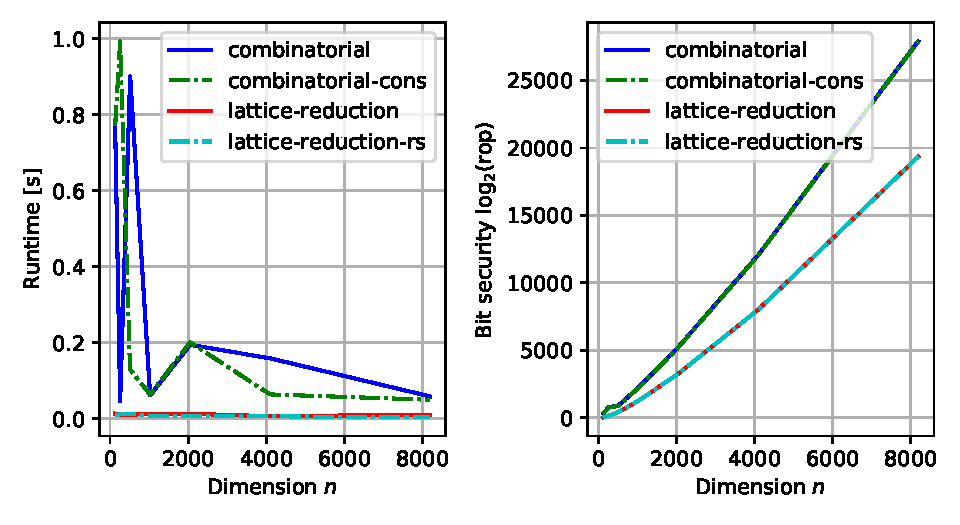
\includegraphics[width=0.8\textwidth]{graphics/SIS_plot.pdf}
        \caption{Large $n$}
    \end{subfigure}
    \begin{subfigure}{1\textwidth}
        \centering
        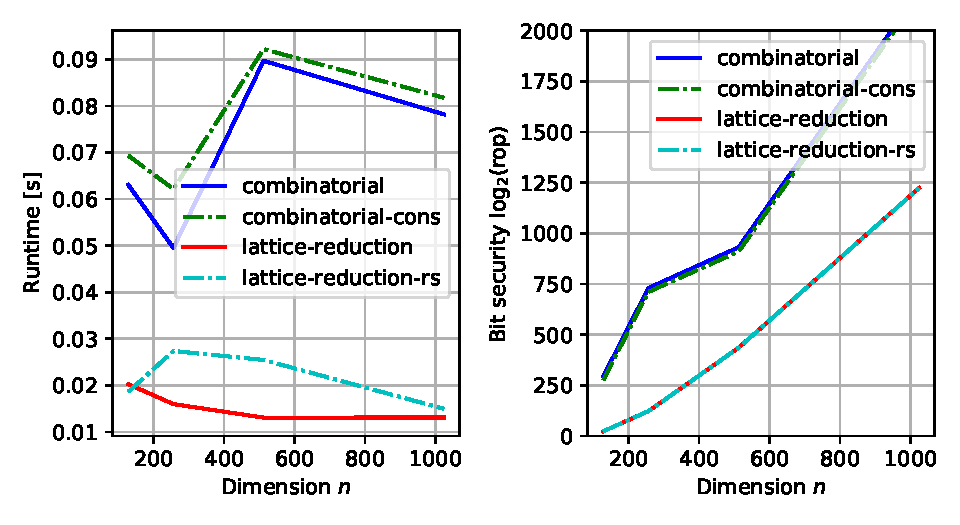
\includegraphics[width=0.8\textwidth]{graphics/SIS_plot_small.pdf}
        \caption{Small $n$}
    \end{subfigure}
    \caption{SIS with $n^2 < q < 2n^2, \; m = 2n \sqrt{n \log q}, \; s = 2 \sqrt{n \log q}$}\label{fig:SIS-algs}
\end{figure}

\begin{figure}[h!]
    \centering
    \begin{subfigure}{1\textwidth}
        \centering
        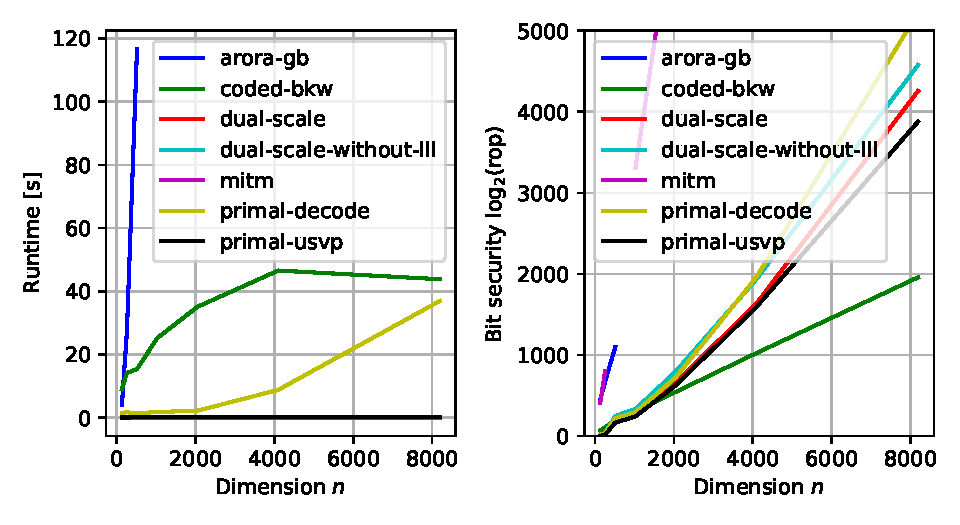
\includegraphics[width=0.8\textwidth]{graphics/LWE_plot_long.pdf}
        \caption{Large $n$}
    \end{subfigure}
    \begin{subfigure}{1\textwidth}
        \centering
        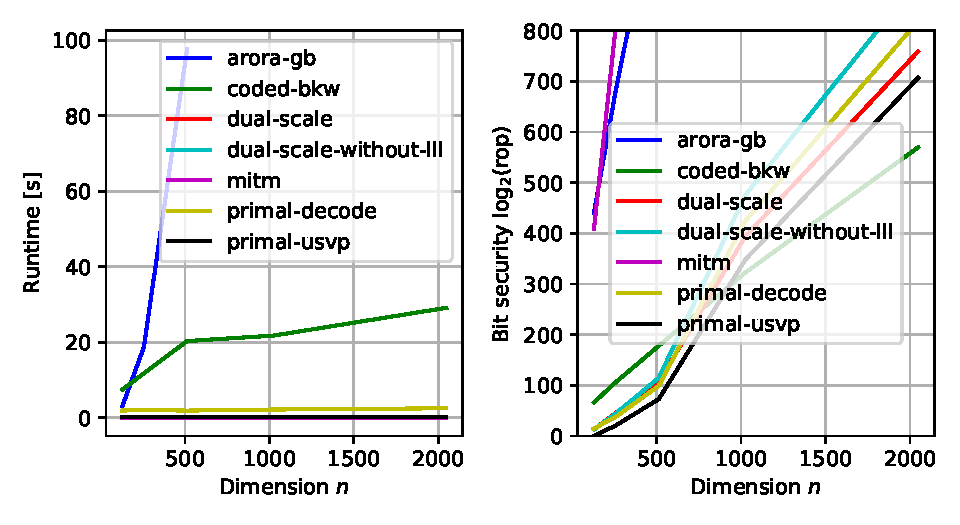
\includegraphics[width=0.8\textwidth]{graphics/LWE_plot_long_small.pdf}
        \caption{Small $n$}
    \end{subfigure}
    \caption{LWE with $\sigma=2.828,\; m=\infty, \; n < q < 2n$}\label{fig:LWE-other-sigma}
\end{figure}
\begin{figure}[h!]
    \centering
    \begin{subfigure}{1\textwidth}
        \centering
        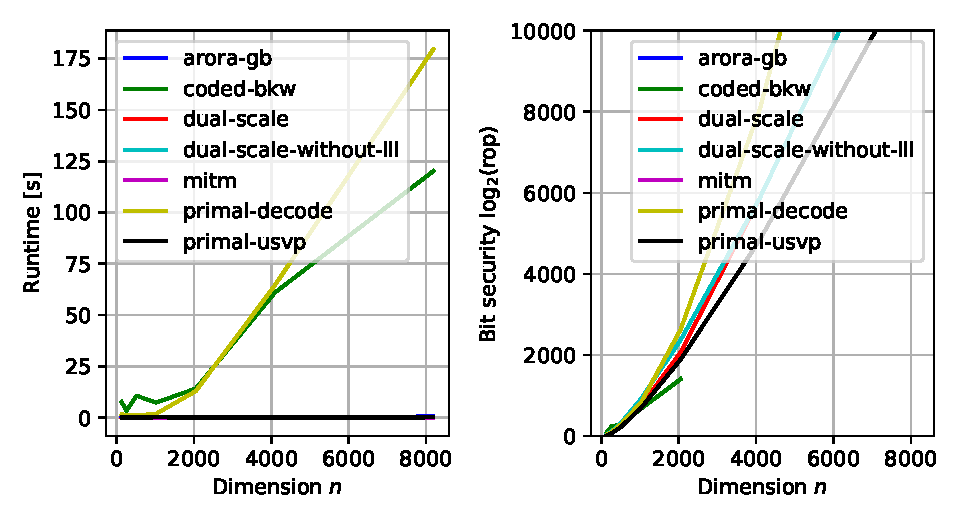
\includegraphics[width=0.8\textwidth]{graphics/LWE_plot_Regev_long.pdf}
        \caption{Large $n$}
    \end{subfigure}
    \begin{subfigure}{1\textwidth}
        \centering
        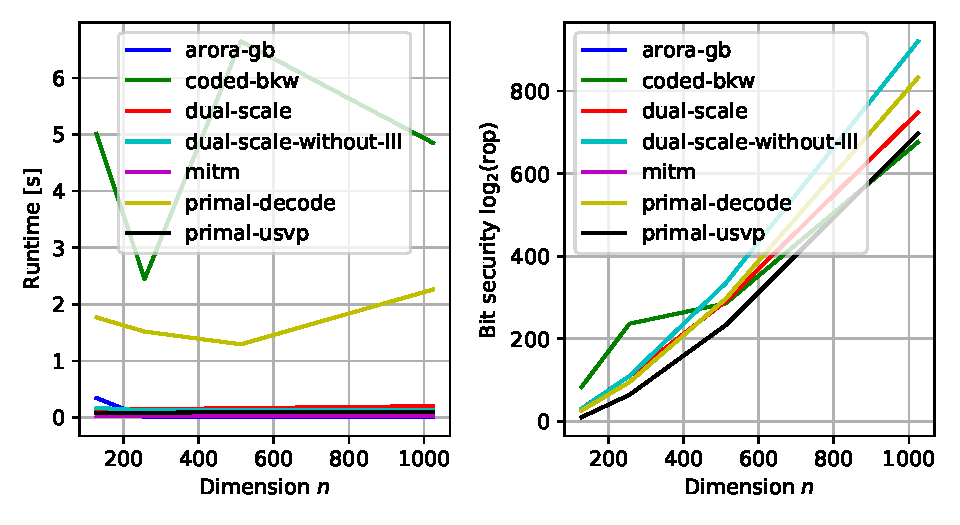
\includegraphics[width=0.8\textwidth]{graphics/LWE_plot_Regev_long_small_n.pdf}
        \caption{Small $n$}
    \end{subfigure}
    \begin{subfigure}{1\textwidth}
        \centering
        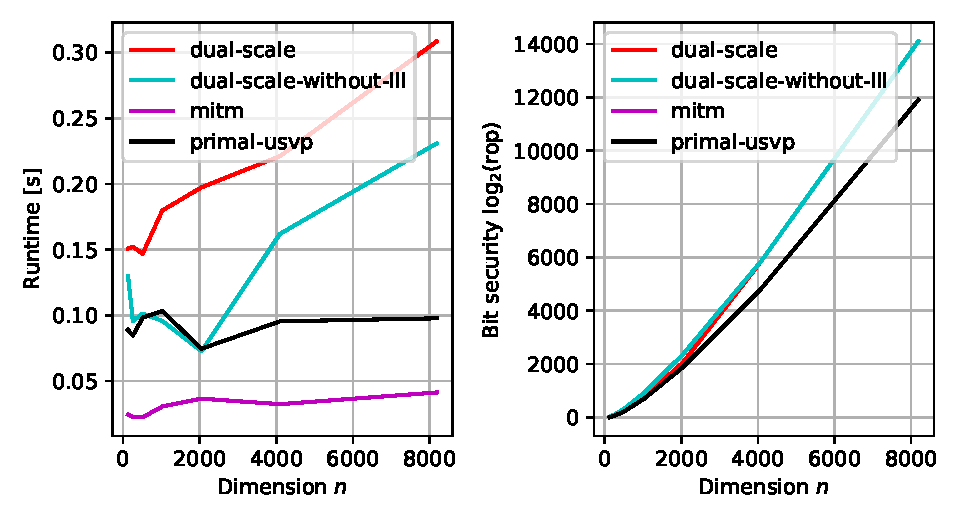
\includegraphics[width=0.8\textwidth]{graphics/LWE_plot_Regev_short.pdf}
        \caption{Only algorithms with short runtime}
    \end{subfigure}
    \caption{LWE with parameters chosen as in \cite{Reg05}}\label{fig:LWE-Regev}
\end{figure}


% TODO: how does dual attack without LLL work???
\begin{table}[h!]
    \centering
    \begin{tabular}[]{lll}
        \toprule
        Algorithm                 & Priority & Justification                                       \\\hline
        Meet-in-the-Middle        & 5        & fastest, high cost estimate, as prefilter           \\
        Primal uSVP               & 10       & fast, low cost estimatate estimates                 \\
        Dual Attack               & 20       & fast, often higher estimates than Primal uSVP       \\
        Dual Attack (without LLL) & 30       & fast, often higher estimates than Dual              \\
        Coded-BKW                 & 90       & slow, somtimes very low cost estimate               \\
                                  &          & (for small stddev), does not always yield results   \\
        Decoding Attack           & 100      & slow, often higher estimates than faster algorithms \\
        Arora-Ge                  & 200      & extremely slow, often higher estimates,             \\
                                  &          & does not always yield results                       \\
        \bottomrule
    \end{tabular}
    \caption{Prioritization of LWE Algorithms}\label{tab:lwe-alg-prio}
    \vspace{1cm}
    \begin{tabular}[]{lll}
        \toprule
        Algorithm                  & Priority & Justification                           \\\hline
        Lattice Reduction MR       & 1        & fastest, low cost estimates             \\
        Lattice Reduction RS       & 2        & same results as lattice-reduction,      \\
                                   &          & not always applicable                   \\
        Combinatorial Attack       & 10       & fast, often higher cost results         \\
        Combinatorial Conservative & 9        & fast, slighly better than Combinatorial \\
        \bottomrule
    \end{tabular}
    \caption{Prioritization of SIS Algorithms}\label{tab:sis-alg-prio}
\end{table}

% TODO first finish section on algorithms
% - include plots
% - write about pro/cons
% - maybe add section of cost comparison for the algorithms of the previous section
\section{Usage Examples}\label{sec:tool-application}
We provide several usage examples in the Python script $\texttt{usage\_example.py}$. A simple estimation example for LWE and SIS show the application of the function $\texttt{problem.estimate()}$ to estimate the security of problem instances for a fixed parameter set. Two simple parameter searches, one for LWE and one for SIS, explain the functionality of the function $\texttt{param\_search.generic\_search()}$. In both cases, as for the algorithm performance analysis in \cref{fig:SIS-algs,fig:LWE-other-sigma}, we derive the parameter choices from \cite{Reg05} and \cite{MP12} for LWE and SIS respectively. % The search for LWE finds paramters $n=512$, $q=262147$, $m=262144$ and $\alpha\approx 0.0005456$ for a bit security level greater than $128$ (the estimates security is $\approx 290$). For SIS, we obtain paramters $n=1024$, $q=1825163$, $m=42597$ and $\beta \approx 1557$, where $\beta$ is in $\ell_\infty$-bound, with an effective security level of $\approx 370$.
In addition, our code includes two more advanced examples for schemes that are currently under research at the Institute of Information Security (SEC), University of Stuttgart. The first is a parameter search for variation of the BGV scheme based on \cite{BGV11,DPSZ12} that ensures accountability. The second finds parameters for a commitment scheme based on \cite{BDLOP18} in an advanced setting and combines LWE and SIS in one search. The examples demonstrate the usefulness of our tool. On the one hand, our tool provides interfaces and default settings that are easy use without much background knowledge. On the other hand, the flexibility of the generic search allows for the combination of multiple primitive building blocks of a complex application, while maintining a simple and clear structure.